\documentclass[12pt]{amsart}
\usepackage{preamble}

\let\PP\P
\newcommand{\PPt}{\mathbb{P}}
\let\P\PPt

\begin{document}
\begin{center}
    \textsc{Math 502. HW 14\\ Ian Jorquera}
\end{center}
\vspace{1em}

\begin{itemize}
%\item[(1)] Notice that $p_q=x_1^q+x_2^q+\dots$ and $p_{(1^q)}=p_1^q=(x_1+x_2+\dots)^q$. Notice that any term in this product that has mixed variables would have a coefficient that has $q$ as a divisor. To see this consider the degree $q$ monomial $m_\lambda$ where $\lambda\neq (q)$  represents the number of distinct variables

\item[(2)] Recall that $h_\mu= \sum_{\lambda}k_{\lambda\mu}s_\lambda$ and so $\ip{h_{(3,2,2)},s_{2,2,1,1,1}}$ is the coefficient of $s_{(2,2,1,1,1)}$ in the above expansion or just $k_{(2,2,1,1,1)(3,2,2)}$ which counts the number of SSYT of shape $(2,2,1,1,1)$ and content $(3,2,2)$ of which there are $0$. This follows from the fact that the content of any filling of (2,2,1,1,1) can never have more then $2$, $1$s but the content $(3,2,2)$ has three $1$s. So $\ip{h_{(3,2,2)},s_{2,2,1,1,1}}=0$.\\

%\item[(5)] To find the character of $V$ we need to consider the permutation matrices of the basis element for each conjugacy class of $S_4$\\

\item[(6)] For some fixed finite field $\F_q$ consider the projective space of $\P^n_{\F_q}$ and its $k$-flats. First notice that the number of points is $v=|\P^n_{\F_q}|=\frac{\F_q^{n+1}-1}{\F_q-1}=\frac{q^{n+1}-1}{q-1}$.
We also know that the number of points in a $k$-flats is counted in the same way $k=\frac{\F_q^{k+1}-1}{\F_q-1}=\frac{q^{k+1}-1}{q-1}$. Notice that any $k$-flat is a $k+1$-dimensional subspace in $\F_q^{n+1}$ of which there are ${n+1\choose k+1}_q$ many. Any two points in the projective space correspond to a $2$-dimensional flat in $\F_q^{n+1}$, and so we must count the number of $k$-flats containing any given $2$-flat. This corresponds to counting the number of $k-1$-dimensional space in $\F_q^{n-1}$, as we remove the plane. And so $\lambda={n-1\choose k-1}_{q}$. And so $(\P_{\F_q}^{n}, \{k\text{-flats}\})$ is a $2$-$(\frac{q^{n+1}-1}{q-1},\frac{q^{k+1}-1}{q-1},{n-1\choose k-1}_{q})$ design, or equivalently a $2$-$({n+1\choose 1}_q,{k+1\choose 1}_q,{n-1\choose k-1}_{q})$ design.\\

\item[(7)] Consider the following deleted Laplacian 
$$\begin{pmatrix}
3 &-1&0&0\\
-1&3&-1&-1\\
0&-1&2&-1\\
0&-1&-1&3\end{pmatrix}$$
Whose determinant is $19$, giving us that there are $19$ maximal spanning tree and therefore $19$ bases.\\
\item[(8)] Below is a drawing of $\P_{\F_3}^2$\\
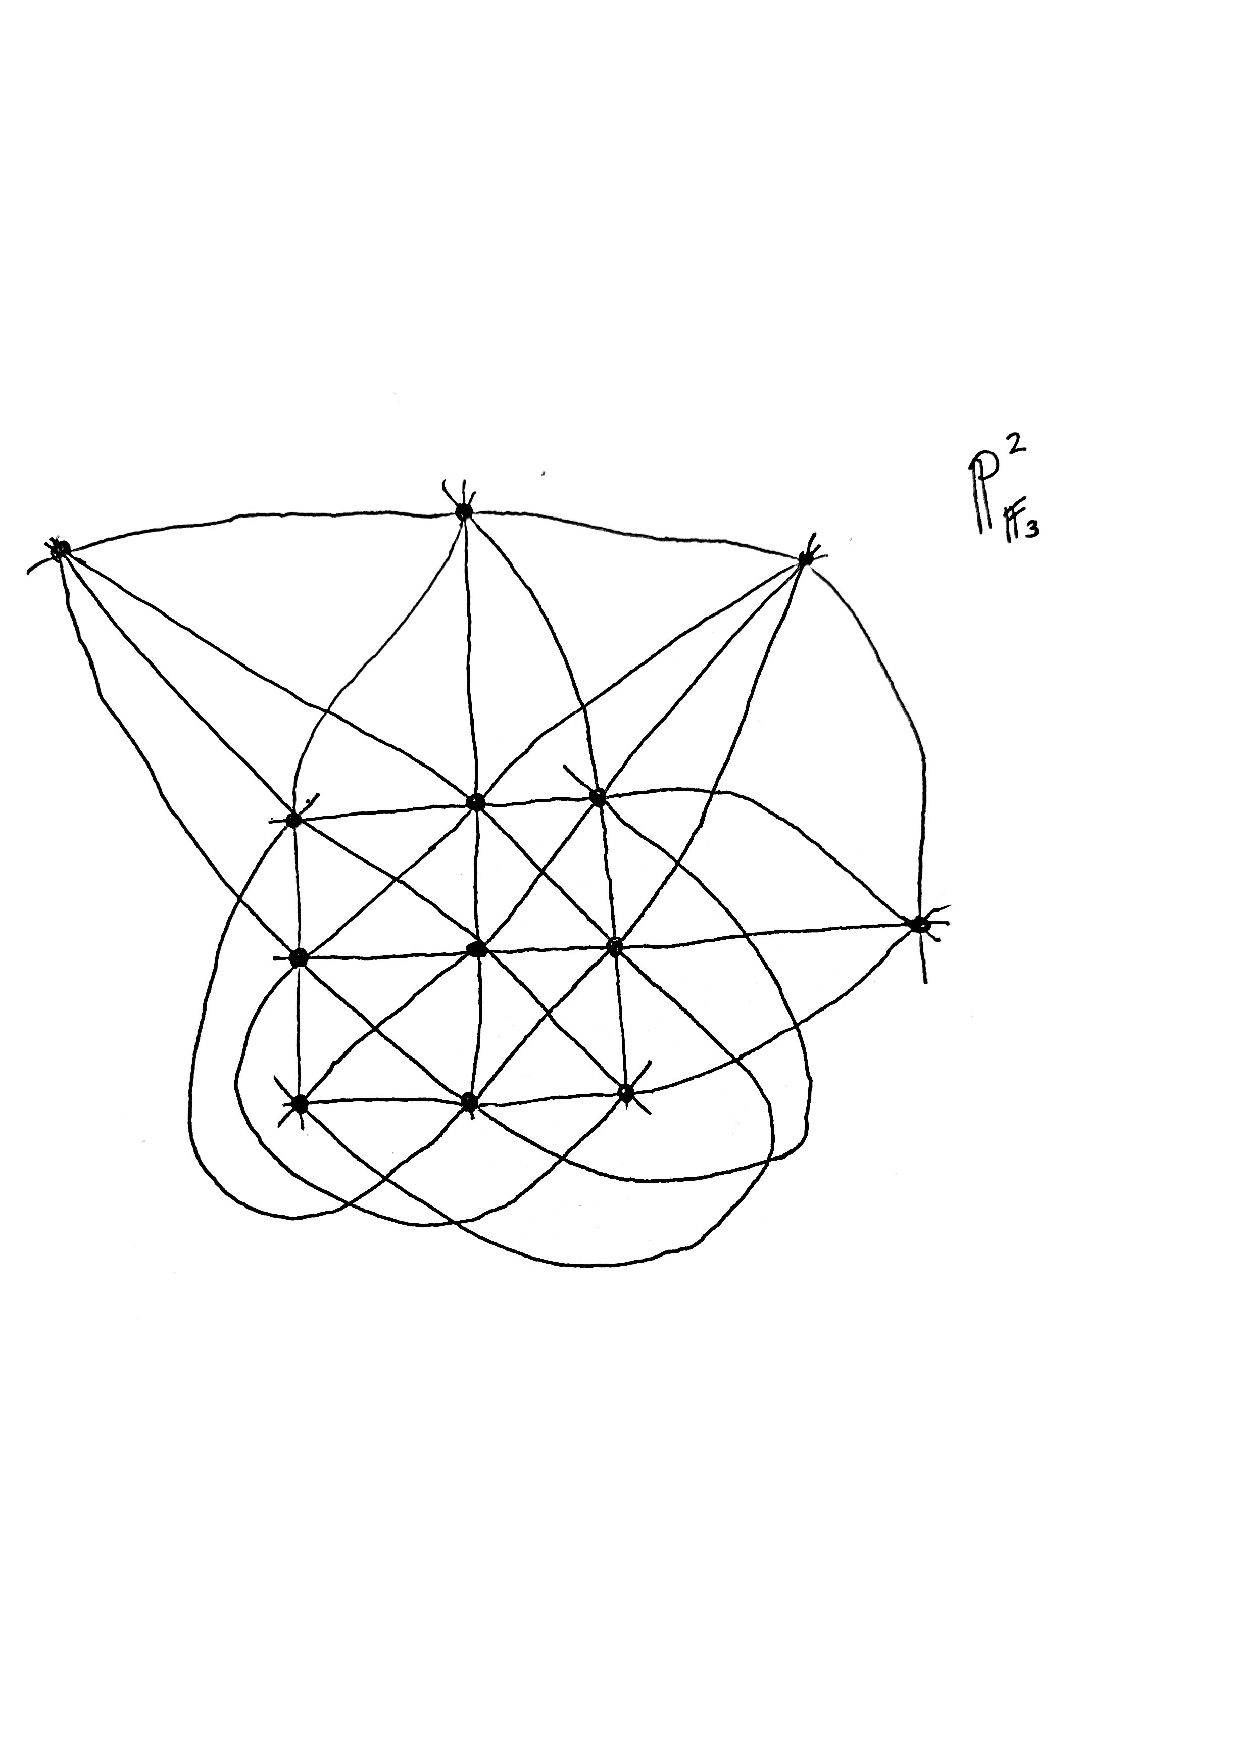
\includegraphics[trim={0 7cm 0 6cm}, scale=.4]{pics/hw14p2f3.pdf}
\item[(9)] This follows from the fact that the orthogonal compliment of a $k$ dimensional subspace in a vector space of dimension $n$ is a subspace of dimension $n-k$. And the orthogonal compliment on subspaces is an involution\\

\item[(10)] Recall that in the chow ring $A^*(\text{Gr}(k,n))$ there is a bijection mapping $\sigma_\lambda\ra s_\lambda$ when ever $\lambda\se ((n-k)^k)$. So in the Chow ring $A^*(\text{Gr}(3,6))$ we can compute the product $\sigma_{(2,1)}^3$ using the truncated Littlewood-Richardson rule on $s_{(2,1)}^3$ ignoring all terms whose partition is not contained in the box $(3,3,3)$. This gives us, using sage that 
$$\sigma_{(2,1)}^3=2\sigma_{(3, 3, 3)}$$
\end{itemize}


\end{document}

